\documentclass[12pt]{article}
\usepackage[utf8]{inputenc}
\usepackage[margin=2cm,includefoot,footskip=30pt,]{geometry}
\usepackage{graphicx}
\usepackage{bold-extra}
\usepackage{graphicx}
\graphicspath{ {imagens/} }
\usepackage{epstopdf}
\usepackage{float}

\usepackage{scalerel}
\usepackage{mathtools}
\usepackage{stackengine}
%\usepackage{xcolor}
\newcommand\showdiv[1]{\overline{\smash{\hstretch{.5}{)}\mkern-3.2mu\hstretch{.5}{)}}#1}}
\newcommand\ph[1]{\textcolor{white}{#1}}

% ----- Cabeçalho e rodapé -----
\usepackage{fancyhdr}
\pagestyle{fancy}
\fancyhf{}

\renewcommand{\headrulewidth}{1pt}
\renewcommand{\footrulewidth}{0.5pt}

\rhead{1º Trabalho Computacional}
\lhead{Matematica Computacional\rightmark}
\rfoot{Página \thepage}
\lfoot{\small Engenharia Electrotécnica e de Computadores - IST}


\usepackage{pdfpages}

\begin{document}


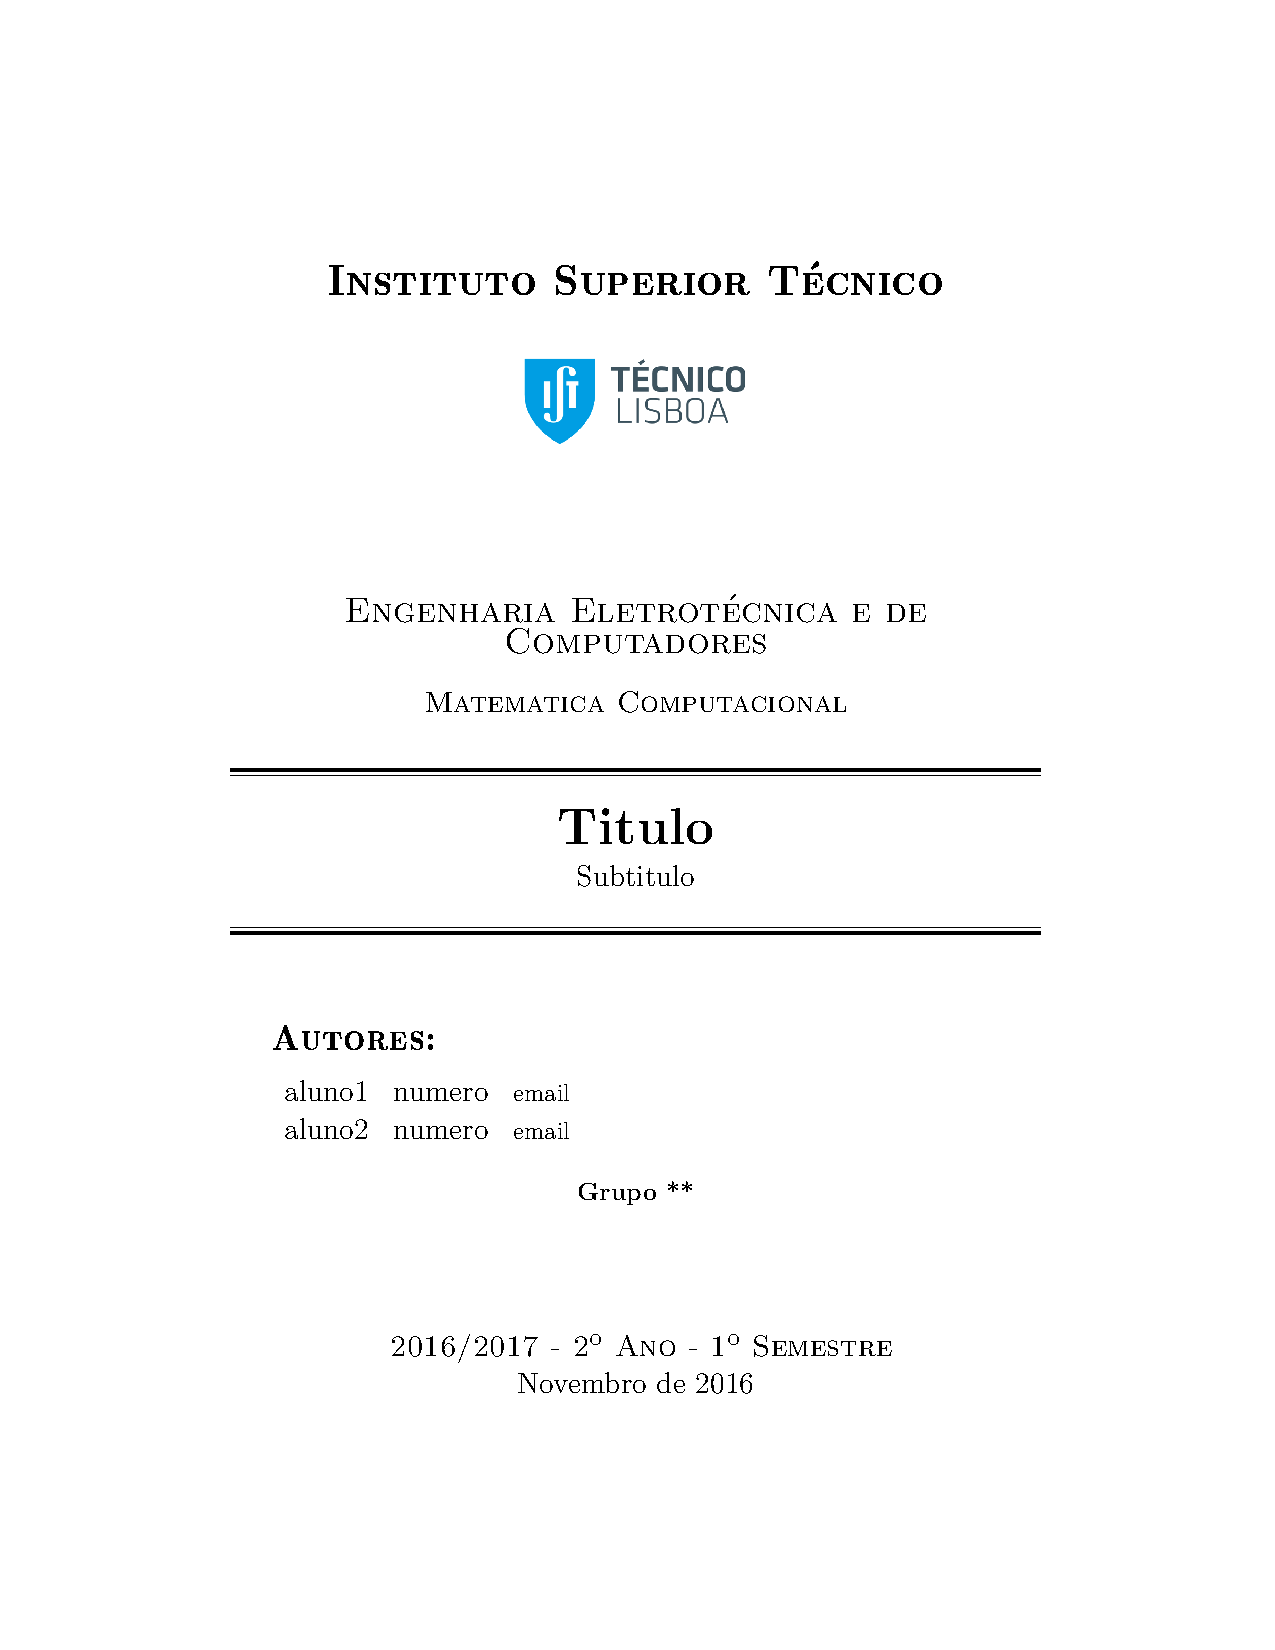
\includepdf[pages={1}]{capa/capa.pdf}

\section{Pergunta 1}
\begin{equation}
	h(\lambda) = \lambda + 15.5 - 2\cosh(\lambda)
\end{equation}
\begin{equation}
	h'(\lambda) = 1 - 2\sinh(\tau\lambda) = 1 - \tau(e^{\tau\lambda} - e^{-\tau\lambda})
\end{equation}
\begin{equation}
	h''(\lambda) = 2\tau^2\cosh(\tau\lambda) = -\tau^2(e^{\tau\lambda} + e^{-\tau\lambda})
\end{equation}

Analisemos o sinal de $h''(\lambda)$:
\begin{equation}
	e^{\tau\lambda} + e^{-\tau\lambda} > 0 \implies h''(\lambda) < 0
\end{equation}

Pelo Teorema de Rolle e pela inequação (4) podemos afirmar que
$h'(\lambda)$ tem no maximo duas raizes.

\begin{equation}
\begin{split}
	\lim_{x \to +\infty} h(\lambda)
	&= \lim_{x \to +\infty} (\lambda + 15.5 - 2\cosh(\lambda)) \\
	&= \lim_{x \to +\infty} e^{\tau\lambda} \bigg(\frac{\lambda}{e^{\tau\lambda}} + \frac{15.5}{e^{\tau\lambda}} - \frac{2\cosh(\lambda)}{e^{\tau\lambda}}\bigg) \\
	&= e^{+\infty} (0 + 0 - 1) = -\infty
\end{split}
\end{equation}

Analogamente para  $-\infty$ :
\begin{equation}
\begin{split}
	\lim_{x \to -\infty} h(\lambda)
	&= \lim_{x \to -\infty} (\lambda + 15.5 - 2\cosh(\lambda)) \\
	&= \lim_{x \to -\infty} e^{-\tau\lambda} \bigg(\frac{\lambda}{e^{-\tau\lambda}} + \frac{15.5}{e^{-\tau\lambda}} - \frac{2\cosh(\lambda)}{e^{-\tau\lambda}}\bigg) \\
	&= e^{+\infty} (0 + 0 - 1) = -\infty
\end{split}
\end{equation}

\section{Pergunta 2}
\subsection{Aliena a)}

\section{secção3}

\section{secção4}

\end{document}
